\documentclass[a4paper,11pt]{article}
\usepackage[utf8]{inputenc}
\usepackage{amsmath}

% set up sensible margins (same as for cssethesis)
\usepackage[paper=a4paper,left=30mm,width=150mm,top=25mm,bottom=25mm]{geometry} 
\usepackage{cite} % Use the natbib bibliography and citation package
\usepackage{setspace} % This is used in the title page
\usepackage{graphicx} % This is used to load the crest in the title page
\usepackage{amsmath}
\usepackage{multicol}
\usepackage{color}
\usepackage{textcomp}
\usepackage{algpseudocode}
\usepackage{algorithm}
\usepackage{amssymb}
\usepackage{cleveref} 
\usepackage{epsfig}
%\usepackage[ruled, vlined]{algorithm2e}
\usepackage{epstopdf}
\usepackage{subfigure}
\usepackage{sectsty} 
\usepackage{amsmath}
\usepackage{qtree}
\usepackage{multirow}
\usepackage{lscape}
%\usepackage{refcheck}
%\usepackage[backref]{hyperref}
%\usepackage{hyperref}
%\usepackage{rotating}
%\usepackage{comment}


%\usepackage{enumerate}
%\usepackage[shortlabels]{enumitem}

\begin{document}


%\begin{enumerate}[start=1,label={(\bfseries Q\arabic*):}]

% Set up a title page
\thispagestyle{empty} % no page number on very first page
% Use roman numerals for page numbers initially
%\renewcommand{\thepage}{\roman{page}}

\begin{spacing}{1.5}
\begin{center}

{\LARGE \bfseries
Political Stance Detection in Posts Across Online Social Networks}
\medskip\\
\textbf{A Report}
\begin{center}
submitted in partial fulfillment of\\ 
the requirements for the award of the degree of\\
\textbf{Bachelor of Technology}
\medskip\\
in\\
\textbf{INFORMATION TECHNOLOGY}\\
\textbf{BY}
\medskip\\
Priyam Bansal (01901032015)\\
Zoya Khan (02001032015)\\
Mansi Sharma (03201032015)\\
\end{center}
\begin{center}
\textbf{Under the Guidance of}\\
\end{center}
%\begin{center}
%Rishabh Kaushal\\
%Assistant Professor\\
%Department of Information Technology\\
%Indira Gandhi Delhi Technical University for Women
%\end{center}
\begin{center}
\textbf{Mr. Rishabh Kaushal}\\
Assistant Professor\\
Department of Information Technology\\
Indira Gandhi Delhi Technical University for Women
\end{center}
\vspace*{10mm}


\includegraphics[height=5cm,width=5cm]{igdtuw_logo.jpg}

{\LARGE \bfseries
Indira Gandhi Delhi Technical University for Women\\
Kashmere Gate, Delhi - 110006\medskip\\
2015-2019
}

\end{center}
\end{spacing}

\newpage
{\LARGE \bfseries CERTIFICATE}
\pagenumbering{roman}
\setcounter{page}{1}
\addcontentsline{toc}{section}{CERTIFICATE}
\vspace*{5mm}
\medskip\\
\begin{spacing}{1.5}
This is to certify that the work presented in this B.Tech. Report titled \textbf{“Political Stance Detection in Posts Across Online Social Networks”} is an authentic record of our own work under the supervision of \textbf{Mr. Rishabh Kaushal, Assistant Professor}, Department of Information Technology. It is submitted in partial fulfillment of the requirements for the award of the \textbf{Bachelor of Technology in Information Technology} at Department of Information Technology, Indira Gandhi Delhi Technical University for Women.

\vspace*{1.70cm}
{\hspace*{\fill} {\textbf{PRIYAM BANSAL\\\hspace*{\fill}01901032015}}}

\vspace*{0.05cm}
{\hspace*{\fill} {\textbf{ZOYA KHAN\\\hspace*{\fill}02001032015}}}

\vspace*{0.05cm}
{\hspace*{\fill} {\textbf{MANSI SHARMA\\\hspace*{\fill}03201032015}}}

\vspace*{1.25cm}
{This is to certify that this work has been done under my supervision and guidance. It has not been submitted elsewhere either in part or full, for award of any other degree or diploma to the best of my knowledge and belief.}

\vspace*{2.5cm}
{\textbf{DATE:}\hspace*{\fill} {\textbf{Mr. Rishabh Kaushal\\\hspace*{\fill}Assistant Professor}}}
\end{spacing}

\newpage
{\LARGE \bfseries ACKNOWLEDGMENT}
\addcontentsline{toc}{section}{ACKNOWLEDGMENT}
\vspace*{5mm}
\medskip\\
 \begin{spacing}{1.5}
    We would like to express our special thanks of gratitude to our project supervisor, \textbf{Mr. Rishabh Kaushal}, Assistant Professor, Department of Information Technology, Indira Gandhi Delhi Technical University for Women. The objective and scope of this project was
    formulated under his guidance and his willingness to
    provide constant feedback to us on our work helped us to
    improve and refine the project. \\
    \\
    Also we would like to thank our Head of Department, \textbf{Dr. Arun Sharma}, Department of Information Technology for giving us the golden opportunity to do this wonderful project in college. 
    
  \vspace*{2.5cm}
{\hspace*{\fill} {\textbf{PRIYAM BANSAL\\\hspace*{\fill}01901032015}}}

 \vspace*{0.1cm}
{\hspace*{\fill} {\textbf{ZOYA KHAN\\\hspace*{\fill}02001032015}}}
 
 
 \vspace*{0.1cm}
{\hspace*{\fill} {\textbf{MANSI SHARMA\\\hspace*{\fill}03201032015}}}
\end{spacing}


\newpage
{\LARGE \bfseries ABSTRACT}
\addcontentsline{toc}{section}{ABSTRACT}
\vspace*{5mm}
\medskip\\
Our project aims at detecting the political stance of people living in and around New Delhi, India who tweet about their political opinions on Twitter. We concentrate our focus on the three major political parties that have been influential in the Delhi political scenario over the past few years namely, Aam Aadmi Party, Bhartiya Janta Party and Indian National Congress.
\medskip\\
We begin by initiating a  manual  collection  of  twitter users who live in and around Delhi and tweet about politically related issues. We identify 248 such users and with the help of Twitter's REST API we collect all (maximum 3,200) tweets from these users. 
\medskip\\
Using Natural Language Processing we build a political filter that filters out politically-related tweets among the whole tweet corpus that might have some out of context tweets too. A random sample of tweets of this data is then manually annotated in binary and multilevel classes according to their inclination towards or against any of the above identified political parties. 
\medskip\\
A Long Short Term Memory unit is trained for text classification to classify a given tweet as politically sensitive or not. This Long Short Term Memory model is trained using the random tweet dataset created in the initial phase and is used to predict the labels for new tweets.

\newpage
\tableofcontents
\newpage

\listoffigures
\addcontentsline{toc}{section}{List of Figures} 
\listoftables
\addcontentsline{toc}{section}{List of Tables}

\newpage
\pagenumbering{arabic}
\setcounter{page}{6}
\section{INTRODUCTION}
\hrule
\vspace*{5mm}

\subsection{Background}
Online Social Networking websites such as Twitter, Facebook, MySpace, Instagram, LinkedIn provide people a means to share their thoughts, connect with old friends and make new ones. The popularity of such platforms is increasing day by day, with people expressing their thoughts with all kinds of media be it personal photographs, the new age memes, articles, videos, polls and open letters, on all kinds of issues be it personal or social and with this there is a bulk of sensitive information revealed by them. 
\medskip\\
One such information leak is encountered while expressing political views on social media platforms. While many users may not think that the political views they share are sensitive to privacy, we argue that even a single post relating to this subject can be used determine their political stance even though the users themselves have never revealed it explicitly on any of these platforms.
\medskip\\
Indian population is actively sharing their political views on online social networks. People are often seen expressing their views on new government policies and other latest developments and raising relevant political issues. Some people outwardly show their support to different political parties and/or leaders while some criticize or troll them. People also issue complaints and show their disappointment on these platforms and even the government bodies, politicians, senior leaders and parties communicate with general public here. When so much information pertaining to this domain is shared actively on online social networks, an individual may unintentionally give cues that can be used to determine his political stance.
\medskip\\
Twitter, a micro blogging website, is the most popular medium to express such thoughts among general public and political and entities alike. India stands third in largest Twitter using population of a country, with an average of 36 million users in 2018 so naturally political parties will reach out to the voters with the help of this powerful platform. Politicians can promote and present their point of view without being prey of media format limitation or being interrupted by journalists during press conference and they can post their presumptive political agenda, giving direct contact to the voters. Twitter has become indispensable in organizing political campaigns. 
\medskip\\
It allows like-minded voters and activists to share news and information such as campaign events in a convenient manner. Political parties or politicians can invite general public to participate in the discussions on issues of public interest. Parties may even try to manipulate people and make them swing towards them by creating a good sentiment for themselves with fake paid accounts and heavy trolling of the rival parties.
\medskip\\
These actions motivate general people to express their own thoughts and views on such matters and sometimes people get carried away and disclose private information unintentionally. This disclosure of political privacy can have serious repercussions like forestalling attempts to influence the voter by intimidation, blackmailing, and potential vote buying. This makes the problem important to solve.
\medskip\\
While sentiment detection has been an ever-present problem, stance detection has only recently started to gain research attention. Stance detection of Indian population poses an added set of concerns with numerous political parties, people with diverse backgrounds practicing different religions and expressing views in different languages.

\subsection{Motivation for Report}

In this digital age, the amount of data that is being generated and consumed is growing exponentially. With this rapid increase, there increases the need for security and privacy of this data.
There are numerous laws in place already that are supposed to protect the privacy of a user in the online realm. These laws are supposed to ensure that privacy breaches of a user do not take place.
\medskip\\
In the global context, the EU GDPR is a ground breaking step taken by the European Union in 2018 towards protection of the data privacy and rights of its citizens.\medskip\\
The European Union Global Data Protection Regulation governs the data privacy across all corporations processing data of residents of the European Union. In order to ensure that this regulation is followed with utmost care, the penalty of non conformance is set at 4\% of the global turnover of the corporation.
\medskip\\
The EU GDPR equips the users by providing them the following basic rights :
\begin{enumerate}
    \item Breach Notification :
    The organization is required to inform its users of any possible breaches that might have occurred within 72 hours of the breach happening.
    \item Right Access : This grants a user the right to ask the organization, how and where their data is being used.
    \item Right to be Forgotten : This grants a user the right to completely delete their data from the organization.
    \item Data Portability : This grants a user the right to ask the organization for all the data related to him/her in a readable format.
\end{enumerate}
In the Indian political scenario, a very recent issue is that of ballot selfies. There is a never ending debate on whether ballot selfies are a breach to privacy or not? In Figure \ref{fig:example1} people are shown holding their Voter ID cards. As can be seen, the text on most of the Voter IDs is legible and hence can be misused by people with malicious intentions. These people are essentially giving away their private information that can be misused in many ways.
\medskip\\
With the ever increasing usage of social media by the Indian population a large number of instances are seen on Twitter where people have lost their jobs/internships due to their tweets. One of the famous example is that of a Cisco new recruit complaining about the travel to work and her hatred for her new job. Figure \ref{fig:example2} shows a snapshot of the thread.
\medskip\\
People express their thoughts on social media which can sometimes lead to privacy breaches. For example, people are not allowed to tell who are they going to vote for in a political election. They might not directly speak but sometimes their tweets can give a strong indication of favoritism towards a particular political party like in Figure \ref{fig:example3} or sometimes a person can be against one party which can be deduced from their tweets like in Figure \ref{fig:example4}.
\medskip\\
All this motivates us to analyze the tweets and their privacy aspect and use the predictive models to classify and predict the nature and trend in tweets related to politics.

\begin{figure}
    \centering
  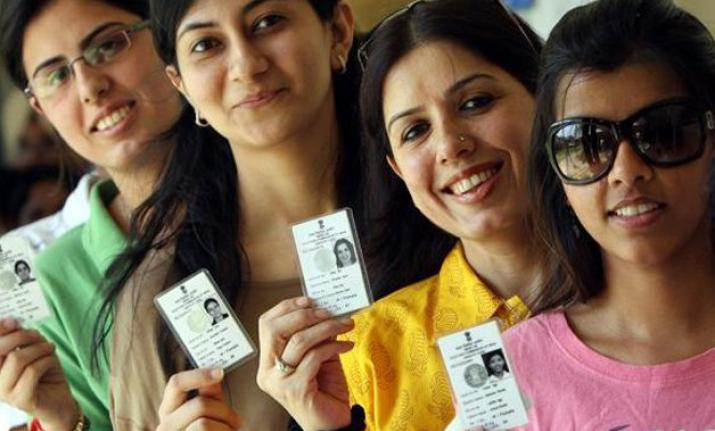
\includegraphics[width=13.5cm]{ballot.jpg}
  \caption{A Ballot Selfie}
  \label{fig:example1}
\end{figure}

\begin{figure}
  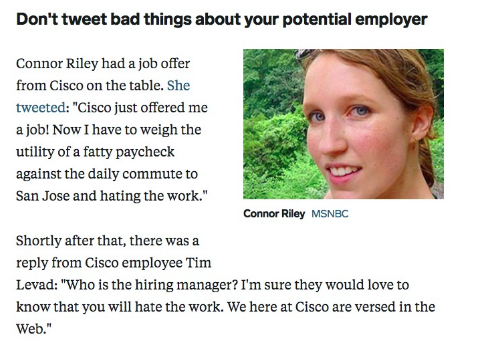
\includegraphics[width=\linewidth]{CiscoTweet.png}
  \caption{Snapshot of a news article about how a girl lost her job}
  \label{fig:example2}
\end{figure}

\begin{figure}
    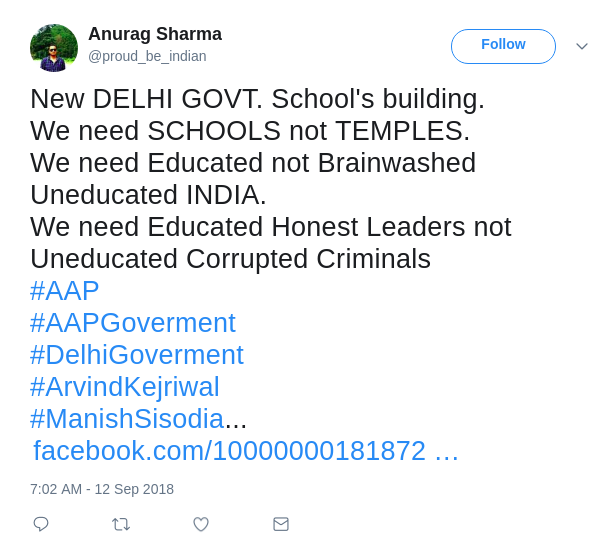
\includegraphics[width=\linewidth]{pro.png}
    \caption{A tweet with positive political stance}
    \label{fig:example3}
\end{figure}

\begin{figure}
    
\includegraphics[width=\linewidth]{anti.png}
    \caption{A tweet with negative political stance}
    \label{fig:example4}
\end{figure}

\newpage
\subsection{Report Outline}

The first phase is the data collection phase in which twitter users residing in and around Delhi/NCR who frequently tweet related to BJP, AAP or Congress are collected via the Twitter API. Tags are manually given based on whether they are in favour, against or undeterministic in their inclination towards a political party. 
\medskip\\
Tweets are collected of these users and stored in MongoDB which this stores JSON data. 
Further, using natural language based political filter is used where we have created a dictionary of words which contains only political related words which are matched against the words in the tweet to extract only the political tweets.\\
The script uses Snowball Stemmer to effectively carry out this process.\\
Stop words and punctuation are deliberately removed as they give no new information and so that they don't divert us from the main problem.
Also, we randomly selected 50 tweets per person for further analysis.
\medskip\\
The tweets are then manually annotated into two classes. The first class defines whether a tweet indicates political inclination or not.\\
The Second class classifies the politically inclined tweets into one of the six following classes: Pro - AAP, Pro - BJP, Pro - Congress, Anti - AAP, Anti - BJP, Anti - Congress.
\medskip\\
Next, classification of the binary class is done using Recurrent Neural Networks. Basically Long Short Term Memory units are used which are a special type of Recurrent Neural Network. These Recurrent Neural Networks have the specialized ability to retain past information and give the output accordingly. It can remember relevant information for a long duration and is therefore our choice as a classifier.
\medskip\\
The accuracy of our Long Short Term Memory unit is 71.7\% on our dataset. Various charts are included in the report for comparison done between accuracies of varying datasets, parameters etc.
\medskip\\
This work is to be extended by improving the accuracy obtained by using different parameters in RNN, by increasing the size of the dataset and by using Word2Vec for better vectorization of words.\\
Also, Integration of Hindi Language tweets and classification of the multi-class (1-6) is to be done.


\newpage
    
\section{PROBLEM STATEMENT}
\hrule
\vspace*{5mm}
\textit{Political Stance Detection in Posts Across Online Social Networks.}\medskip\\
Online Social media platform in focus : Twitter.\\
Aim : To extract tweets related to \textit{political views} and to determine and predict the political inclinations of Twitter users living in and around New Delhi, India.
\medskip\\
In order to detect the political stance of users we use a Long Short Term Memory unit, which are a special type of Recurrent Neural Networks used frequently for text classification.
\medskip\\
The project begins with manual identification of 248 Twitter users and then collection of all (maximum 3,200) tweets of these users. We use Natural Language Processing to filter out the tweets and select only the ones related to politics. A random sample of this data is then manually annotated in binary and multi-level classes according to the users inclination towards or against the aforementioned three political parties namely, Aam Aadmi Party, Bhartiya Janata Party and Indian National Congress.\\
\medskip\\
A Long Short Term Memory unit is trained for text classification to classify a given tweet as politically sensitive or not. This Long Short Term Memory model is trained using the random tweet dataset created in the initial phase and is predict the labels for new tweets.

\newpage
\section{LITERATURE REVIEW}
\hrule
\vspace*{5mm}
Online Social Media are increasingly becoming popular as a field of study and analysis of data. People sometimes reveal a little too much about themselves through their posts which leads to breach of their privacy. Many researches are trying to determine the cause and the related outcome associated with these.
\medskip\\
Diane et. al. \cite{gan2015social} give us a detailed explanation about how one can unintentionally provide information on social media like through posting of their location, which can be misused and hence reveal private information which can have considerable implications. This helps us to realize the importance of privacy and various dangers associated with posting content on social media.
\medskip\\
Mathias et. al \cite{humbert2013nowhere} provide an interesting study about our profiles on social media that they are always vulnerable to attack whatsoever privacy setting we might have in our accounts. They explain the procedure and algorithm an attacker might use to find information about a certain individual. This reveals that once we have a digital footprint, our information can be accessed by unauthorized people. 
\medskip\\
Huina et. al \cite{mao2011loose}  And Wang et. al \cite{wang2011regretted} form the basis for our motivation as here they give detailed findings on privacy leaks on twitter and the latter analyze regrettable tweets. Furthermore, tweets like the infamous Cisco incident where a new employee got fired due to her insensitive tweet added to the motivation.
\medskip\\
We are currently focusing our study on politically inclined tweets. Lu et. al \cite{zhou2016tweet} extract only English Tweets using the Twitter Streaming API using the ‘en’ filter which we implement in our python code for them same purpose. There are tweets which they exclude as they are of no significance like tweets deleted because of typos, rephrasing etc. which are of no relevance to their aim. Similarly we excluded some people from our study have used NLTK based approach by using snowball stemmer to try and extract only the politically related tweets.
\medskip\\
The main aim of the study of Lu et. al \cite{zhou2016tweet} is to analyze and identify deleted tweets and  from them get the regrettable ones. They use various classes for their analysis. Also, Huina et. al \cite{mao2011loose} filter data into classes like vacation tweets, drunk tweets etc. from these we get an idea to classify our tweets into various political classes for better analysis.
\medskip\\
Anna et. al \cite{stavrianou2014nlp} predict opinions in the political reference for tweets regarding politicians using natural language processing and machine learning techniques. They take two categories, one which depicts opinion polarity and the other which does not. It aims to improve by doing multi-class labelling. In the same vein we currently classify our tweets into 1 and 0 the former depicting political inclination of the tweet and the other does not and classify and predict the same using NLP techniques.
\medskip\\
Vishal et. al \cite{kharde2016sentiment} thoroughly describe and present the model and implementation of sentiment analysis of the tweets to classify them into positive or negative. They present two approaches – one is the machine learning and the other lexicon based approach. They describe sentiment analysis as a challenging task which involves natural language processing, machine learning techniques and web mining. They decompose this task into various tasks and explores each one of them. They provide detailed information about the 4 levels of sentiment analysis and finally produce results of the analysis using different algorithms. 
\medskip\\
Taking inspiration from Vishal et. al \cite{kharde2016sentiment}, Mohit et. al \cite{iyyer2014political}  give us a deep insight for classifying tweets in the political domain using Recurrent Neural networks. This forms the basis of our work. Mohit et. al \cite{iyyer2014political} list the properties of RNN which are very effective in detecting the bias in tweets and give us an idea behind the working of a standard RNN model. They list 2 options for initializing the parameters and demonstrates that choosing word2vec over random initialisation provides better results. They used the crowdflower platform their annotating their tweets into either liberal or conservative. In our work we do manual annotation of tweets as no such platform is available for the Indian political scenario. Further, we have applied RNN for classifying the tweets into either politically inclined or not. We aim to improve this by incorporating the word2vec technique. 
\medskip\\
Daniel et. al \cite{preoctiuc2017beyond} move beyond the 2 class labelling to 7 pt. scale labelling. They classify the tweets of the users who are asked to rate their political inclination on the Qualtrics platform and also asked to submit their twitter accounts from which, after verifying that the accounts are genuine, tweets are extracted for dataset construction. They use linguistic features like word2vec, LIWC and unigrams in their analysis. We aim to extend our work by incorporating this multi-labelling and using word2vec for better results. 
\newpage

\section{DATA COLLECTION}
\hrule
\vspace*{5mm}

\subsection{Manual Identification of Twitter Users}
Our aim is to collect users for political views classification using supervised learning.
We select users residing in Delhi/NCR locations so as to limit the area of interest and build a model for a particular region.
\medskip\\
We consider 3 major political parties –
\begin{enumerate}
    \item BJP
    \item Congress
    \item AAP
\end{enumerate}
\medskip
\medskip
\textbf{Details:}
\begin{enumerate}
    \item Start Date of data collection: 20th September 2018.    \item Frequency of data update: Daily.
    \item Contributors: Members of the group.
    \item Data collected so far:  nearly 250 users.
\end{enumerate}
\textbf{Process:}
\medskip\\
We search for the target users by tweets which contain certain hashtags. Some hashtags that we use - \#BJP, \#AAP, \#Congress, \#Politics, \#Elections etc. This hashtag based search on Twitter gives users which are interested in politics and tweet about the same. We filter these users on the basis of location and language and set the location to only Delhi/NCR regions using the Twitter platform’s location filter capability and language to English using the Twitter platform's language filter capability.\\
To understand the distribution of the sample and have equal number of users for each category we analyze the tweets of these individuals to determine which political party they support or are against and then categorize them in one of the following categories:
\begin{enumerate}
    \item Pro AAP: Tweets indicate that user supports Aam Aadmi Party
    \item Pro BJP: Tweets indiacate that user supports Bhartiya Janata Party
    \item Pro Congress: Tweets indicate that user supports Indian National Congress
    \item Anti AAP: Tweets indicate that user opposes Aam Aadmi Party
    \item Anti BJP: Tweets indicate that user opposes Bharatiya Janata Party
    \item Anti Congress: Tweets indicate that user opposes Indain National Congress
    \item Undeterministic: Tweets can not determine user's political stance
\end{enumerate}
All this data is manually collected in an excel sheet along with the username of the person. We use https://tweeterid.com/ for conversion of the username to the user id for processing of data in the future. The following user accounts are not incorporated:
\begin{enumerate}
    \item Politicians
    \item Media and News Profiles
    \item Residents outside Delhi NCR
    \item Verified Profiles
\end{enumerate}

\begin{table}[!htbp]
\centering
\caption{Distribution of users identified across political parties} 
\begin{tabular}{|p{10cm}|p{2cm}|} 
\hline
 Political Party Classification & No. of People \\
 \hline \hline
 Undeterministic & 71 \\ 
 \hline
 Anti - AAP & 9 \\
\hline
 Anti - BJP & 16 \\
\hline
Anti - Congress & 9 \\
\hline
Pro - AAP & 57 \\
\hline
Pro - BJP & 42 \\
\hline
Anti - Congress & 40 \\
\hline
\end{tabular}
\label{tab:partyDistribution}
\end{table} 

\begin{figure}
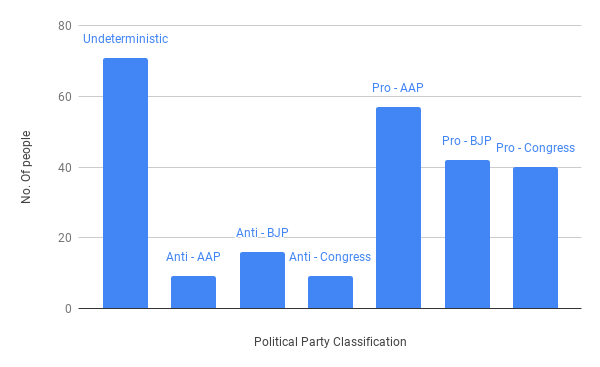
\includegraphics[width=\linewidth]{chart.png}
\caption{Distribution of users identified across political parties}
\label{fig:partyDistribution}
\end{figure}

\subsection{Collecting Tweets From Users}

After manually identifying users and self labelling them, we download the twitter timeline of these users. Twitter provides Twitter API to interact with their service. Twitter offers two kinds of APIs, a REST API and a STREAMING API. As we want to collect past tweets of users and hence want access to historic data, we use the REST API.
\medskip\\
The Twitter API is a set of URLs that take parameters which let you access many features of Twitter, such as posting a tweet or finding tweets that contain a word etc. \\
One such parameter is the screen\_name which is the unique Twitter username of the user. We use this parameter to extract all the tweets of all the users identified manually.  
\medskip\\
There are a host of Python based clients that allow us to work with this API, one of which is Tweepy which we use, due to its ease of use and simple structure. Tweepy provides the convenient Cursor interface to iterate through different types of objects - Tweets, Users, Entities and Places. Access to each returns a JSON-formatted response and traversing through information is very easy in Python. 
\medskip\\
Since we want the full data returned by the API and the API returns the data in the form of JSON, we store the tweets in MongoDB which is a NoSQL database as for this we won’t need to create all the columns as done in RDBMS systems. MongoDB provides a faster query response and can be clustered easily. Also, if the API changes in future, we would not have to change the structure of the database.
\medskip\\
We use Tweepy to collect the twitter timelines of all the users with a language filter that allows only "English Language" tweets of the user to be stored in the database. To ensure that rest API does not give truncated tweets, we take the tweet mode as extended in the Cursor function to get "full\_text" instead of "text" in the JSON. The retweets though, are still truncated in the "full\_text" and the extended version is available in "retweeted\_status" so the "full\_text" is replaced by that present in "retweeted\_status". After this we have 7,87,000 tweets with us stored in the database.
\vspace*{5mm}

\newpage

\section{NATURAL LANGUAGE BASED POLITICAL FILTER}
\hrule
\vspace*{5mm}
An extremely important aspect of efficient machine learning models is having the right data in the right format so that the algorithm can learn the subtleties of the data and predict with improved precision and accuracy.
\medskip\\
We are dealing with a huge amount of twitter data and not all the tweets that we have captured have a political context.
In order to concentrate our focus only on tweets with some politic context and capture these tweets we create a natural language based political filter to extract only politically relevant tweets from the 8,00,000 tweet corpus that we have.
\medskip\\
Our political filter reduces these 8,00,000 tweets into 40,000 tweets. We are aware that this filter is not fool proof and that some out of context tweets may have crept in, but still it is efficient in reducing our data set size from a whopping 8,00,000 to 40,000.
\medskip\\
To create this filter we begin by creating a comprehensive dictionary of keywords that are usually used in the context of Indian Politics. A Snowball Stemmer is then used to stem these keywords to their word roots. 
\medskip\\
A stemmer stems the word given as input to its word root. For example, consider we have the words "environment", "environmentalist", "environmental" since all these words belong to the same word root, all of them get stemmed to the word "environ". This is increasingly useful when creating systems that don't require an exact key word matching.
\medskip\\
There are three types of Stemmers, Lancaster, Porter and Snowball. We are using the Snowball Stemmer as it is not a extreme Stemmer and stems to the word roots more closely as compared to the others. 
\medskip\\
For example, a Lancaster Stemmer will stem "nature" and "national" both to "nat". This is a very critical issue and because of this we have used the Snowball Stemmer which is comparatively mild and reduces "nature" and "national" to different word roots.
\medskip\\
We tokenize the tweet data and after removing all punctuation and stop words we run a similar Stemmer on these tokens. We then run a keyword matching routine that marks each tweet that had any of these politically oriented words as its contents.
\medskip\\
Removing of stop words and punctuation is a critical process as these provide no new and vital information and hence can be dropped so that the whole focus can be given to the word tokens.
\medskip\\
All further processing and annotations are done only on these marked tweets.
\medskip\\
Here is a list of some of those keywords : \medskip\\
("political","bjp", "aap", "inc", "kejriwal", "kejrival", "modi", "namo", "raga", "pm", "hindutva", "congressi", "bhakt", "aaptard", "aapian","politics", "congress", "rss", "RahulGandhi" , "Yogi", "election","gov", "government", "modiji", "opposition", "nda", "delhi", "upa", "sisodia", "political", "public", "state", "jaitley", "army","party", "government", "vote", "rights", "ballot", "rafale", "corruption", "evm", "court", "demonetisation", "constitution")


 
\newpage
\section{MANUAL ANNOTATION OF TWEETS}
\hrule
\vspace*{5mm}

We aim to build two types of classifiers, a binary classifier to classify the political tweets as "sensitive" and "not sensitive", and one multi-class classifier to classify which political party the sensitive tweet talks about. By sensitivity of a political tweet we mean whether it can be said, by just reading the tweet, that the speaker is disclosing which political party it supports or is against. This may be correlated with the fact that in near future, the speaker will vote for that party in elections, or that he/she is a hardcore supporter or criticizer of that party.
\medskip\\
To build these classifiers, we need to have a training sample that is already labelled, and for that we need to manually annotate this data. Though, we are currently working on the binary classifier, the annotation process should be conducted for both the classifiers together to maintain coherency and avoid bias.
\medskip\\
Process:
\medskip\\
We selected a random set of political tweets that are used for manual annotation, training and testing of the classification models. To have an equal distribution of the number of tweets of each user in the sample, we randomly select 50 political tweets from each user. If a user has less than 50 political tweets, we take all his political tweets. All the tweets are shuffled up and given to the annotator. The annotator is given access to only the "full\_text" of the tweet and no other information about the user like his name, profile link, twitter bio etc. This is done to ensure that the annotation is done by only analyzing the text of the tweet.\\
We annotate these tweets into the following categories:
\begin{enumerate}
    \item Label 1: To classify a sentence as showing the political allegiance of the speaker of sentence (sensitivity):
    \begin{itemize}
        \item 0: not sensitive
        \item 1: sensitive 
    \end{itemize}
    \item Label 2: If the value of label 1 is 1, then which political party is the speaker referring to and in what light:
    \begin{itemize}
        \item 1: Pro AAP
        \item 2: Pro BJP
        \item 3: Pro Congress
        \item 4: Anti AAP
        \item 5: Anti BJP
        \item 6: Anti Congress
    \end{itemize}
\end{enumerate}

The guidelines for annotations for Label 1 are:
\begin{enumerate}
    \item Only the sentence is taken into consideration for the annotation process and the annotator is not given access to any detail of the speaker.
    \item A sentence can be annotated only if it is in English.
    \item The links present in the sentences have to be ignored by the annotator.
    \item Sentences addressing only AAP, Congress and/or BJP are to be annotated. If a sentence addresses any other political party besides these three, it is labelled 0. However, if a sentence has a mention of any other political party, but also consists of a mention of AAP, BJP and/or Congress, it will be annotated.
    \item If a sentence indicates the speaker's political preference or allegiance, the sentence is marked 1.
    \item If a sentence indicates that the speaker is against a political party, the sentence is marked 1.
    \item If a sentence is a general statement about politics or a politician and does not reveal anything about his/her support or criticism of any party, it is marked 0.
    \item If the speaker of a sentence supports a political figure but not the party he/she is associated with, we can not conclude that the person supports the party. Such a sentence is labelled 0.
    \item If the speaker of a sentence criticizes a political figure but not the party he/she is associated with, we can not conclude that the is against the party. Such a sentence is labelled 0.
    \item If the speaker praises or criticizes a government policy and does not comment about any party in his sentence, the sentence is labelled 0.
    \item Any statement about any non political organization connected to any political party, for example RSS, is labelled 0.
\end{enumerate}

\begin{table}[!htbp]

\caption{Some Examples where Label 1 is marked 1}
\centering
\begin{tabular}{|p{12.25cm}|p{1cm}|} 
\hline
 Tweets & Label \\
 \hline \hline
 "Why don’t you put the unedited tapes online @republic? If it was anyone with money, there’d be a defamation case against the \#FakeNews outfit. Republic TV is dumbing our nation down and causing radicalisation. I say this even though the channel is pro \#BJP. https://t.co/J73cXNfnCy" & 1 \\ 
 \hline
 "This happened when u elect DUMB \#OurPMissoDUMB" & 1 \\  
\hline
\end{tabular}
\label{tab:lab1}
\end{table}

\begin{table}[!htbp]
\caption{Some Examples where Label 1 is marked 0}
\centering
\begin{tabular}{ | p{12.25cm} | p{1cm}|} 
\hline
 Tweets & Label \\
 \hline \hline
 
"@TimesNow Shashi Tharoor knows his wife's murder case is closing \&amp; his role in the murder will be exposed- This is a tested evil strategy- Go make anti-Hindu, communal and anti-India comments and when he is convicted and jailed he will claim political vendetta" & 0 \\
\hline
 
 "@AmaninderZ @sprakaashbjp @DeShobhaa Politics was never clean not because of politicians, coz they are one of us.. Its their wickd thoughts" & 0 \\ 
 \hline
 "@thekiranbedi People like you are needed in national politics. We bank on you!" & 0 \\  
\hline

"\#Demonetisation did cause distress but was a huge one-time shock to the black money economy Alongwith \#GST (the biggest systemic reform since 1947), lasting impact on formalising economy Still not sure? Just check status of cash-based business models eg. real estate, pvt edu etc https://t.co/DYz0EmPLem" & 0 \\  
\hline

\end{tabular}
\label{tab:lab0}
\end{table}

\newpage
The guidelines for annotations for Label 2 are:
\begin{enumerate}
    \item Only statements with Label 1 as '1' are to be annotated.
    \item The statement is given Label 2 as soon as it is given Label 1 i.e labelling of one sentence for both the categories should be done in one pass by the annotator.
    \item If a speaker of the sentence is favouring, praising or showing support to Aam Aadmi Party (AAP) it is labelled 1. 
    \item If a speaker of the sentence is favouring, praising or showing support to Bhartiya Janata Party (BJP) it is labelled 2.
    \item If a speaker of the sentence is favouring, praising or showing support to Indian National Congress it is labelled 3. 
    \item If a speaker of the sentence is criticising or trolling Aam Aadmi Party (AAP) it is labelled 4. 
    \item If a speaker of the sentence is criticising or trolling Bhartiya Janata Party (BJP) it is labelled 5. 
    \item If a speaker of the sentence is criticising or trolling Indian National Congress it is labelled 6. 
    \item If a sentence fits a pro category (1,2 or 3) as well as an anti category (4,5 or 6), it is marked with the pro category label i.e either 1,2 or 3.
    \item If a sentence fits in more than one pro category labels it is not annotated and marked 0 in Label 1.
    \item If a sentence fits in more than one anti category and none of the pro categories, it is not annotated and marked 0 in Label 1.
    \item If a sentence fits in more than one anti category and also in one pro category, it is given the pro label i.e 1,2 or 3.
    \item If a sentence means that the speaker is against a party, the annotator can not infer that he/she supports the other party until and unless it is mentioned in the text of the statement and vice-versa.
\end{enumerate}

\begin{table}
    \centering
    \caption{Some Examples of Label 2 annotation}
\begin{tabular}{ | p{12.25cm} | p{1cm}|} 
\hline
 Tweets & Label \\
 \hline \hline
"New DELHI GOVT. School\'s building. We need SCHOOLS not TEMPLES. We need Educated not Brainwashed Uneducated INDIA. We need Educated Honest Leaders not Uneducated Corrupted Criminals \#AAP \#AAPGoverment \#DelhiGoverment \#ArvindKejriwal \#ManishSisodia... https://t.co/jRqNnScZP5" & 1 \\ 
 \hline
"Save this. Frame this. Narendra Modi\'s historic \#AbkiBaarModiSarkaar win heralded on countless front pages. http://t.co/ZX9xF0gj7B" & 2 \\  
\hline
"\@Mnomics \@rockyindian7 \@AAPVind \@alamgirizvi \@jayambadi \@logicalindianz \@BreakiNews \@RafaleScam \@SkepticHindu \@DickDarryl \@KilaFateh \@INCIndia They don’t have any heritage any history, whatever RSS has is full of blood; hatred, so it’s very easy to make fun of someone whose entire lineage has laid down their lives for this country." & 3 \\

\hline
"\#KejriDiwas AAP ditched the people of Delhi by bringing down its Government to take the plunge in the national political arena" & 4 \\

\hline
"The \#BJP \&amp; \@IASassociation have colluded to sabotage the image the \@ArvindKejriwal/\#AAP Govt has built over the years. They have total disregard 4 democratically elected representatives. \#Modi ji, dont punish the Delhiites bcz they chose Kejriwal over u. \@attorneybharti https://t.co/3qVpYD5LQ0" & 5 \\

\hline
"\@Goldiepandey26 \@GetRidofDevils Absolutely true. Its established fact. Basic problem is that \#RahulGandhi is in illusion that he is prince of \#NehruGandhi dynasty n has birth right to rule India.His sycophants never tell him that India is under democracy and he is nothing more than comedian." & 6 \\
\hline
\end{tabular}
\label{tab:lab2}
\end{table}

\newpage
\section{METHODOLOGY}
\hrule
\vspace*{5mm}
\subsection{CLASSIFICATION USING RECURRENT NEURAL NETWORK}
\begin{figure}[ht]
    \centering
    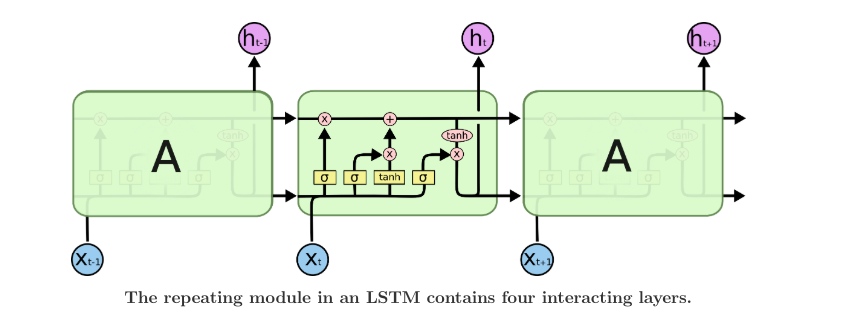
\includegraphics[width=\linewidth]{x.png}
    \caption{Architecture of a LSTM unit}
    \label{fig:my_label}
\end{figure}


The equations that govern the functioning of a Long Short Term Memory unit are :

 \begin{equation}
     \gamma_F^{<t>} = \sigma(W_F  [a^{<t-1>}, x^{<t>}] + b_F)
 \end{equation}
 \begin{equation}
     \gamma_U^{<t>} = \sigma(W_U  [a^{<t-1>}, x^{<t>}] + b_U)
 \end{equation}
 \begin{equation}
     \overline{c}^{<t>} = tanh(W_C[a^{<t-1>}, x^{<t>}] + b_C)
 \end{equation}
 \begin{equation}
     c^{<t>} = \gamma_F^{<t>} * c^{t-1} + \gamma_U^{<t>} * \overline{c}^{<t>}
 \end{equation}
 \begin{equation}
     \gamma_O^{<t>} = \sigma(W_O  [a^{<t-1>}, x^{<t>}] + b_O)
 \end{equation}
 \begin{equation}
    a^{<t>} = \gamma_O^{<t>} * tanh(c^{<t>})
 \end{equation}
 


\[Here,  \gamma_F^{<t>}, \gamma_U^{<t>}, \gamma_O^{<t>} \]  are  the  three gates, Forget, Update and Output respectively. 
\[c^{<t>}, a^{<t>}  \] are the cell state and activation value that is being output by the Long Short Term Memory unit, tanh is the tan hyperbolic function that outputs values in the range of [-1, 1] and sigma is the sigmoid activation function which has the range [0, 1] .
\medskip\\
We are dealing with a huge political corpus of 10,000 tweets from 258 users.
We are building a first level classifier that classifies the given text input as being political orientation revealing or not. 
\medskip\\
A label of 1 indicates that the tweet is revealing the users political orientation and partisan allegiances and a label of 0 corresponds to a tweet that is generic to the political scenario and doesn't reveal the users' political allegiances.
\medskip\\
A specialized neural network, having multiple loops which gives it an edge over traditional neural networks in a manner such that they have the power to remember past events and predict output accordingly is called a Recurrent Neural Network.
\medskip\\
Recurrent Neural Networks are increasing being used in text classification and language modelling tasks everyday and are showing brilliant results in these fields.
\medskip\\
Long Short Term Memory units are a special type of Recurrent Neural Network. These Recurrent Neural Networks have the specialized ability to retain past information and give the output accordingly. It can remember relevant information for a long duration and is therefore our choice as a classifier.
\medskip\\
As is illustrated in the figure, we have five activation functions that are being used and there four internal layers in each LSTM unit. Each of these four layers plays a vital part in the learning and retaining aspect of the long and short term memory unit.
\medskip\\
There are three major gates which govern the functioning of the Recurrent Neural Network, namely Forget, Update and Output gate and as the name suggests, the Forget gate uses a binary sigmoid function and outputs either a 0 or 1 value depending on if the past information is to be remembered or not, if not the forget gates takes the values of 1 and the cell state gets updated by the value of the Update gate, otherwise, the cell state retains its past value. A new cell state and final activation is calculated using the tan hyperbolic activation function.
\medskip\\
The loss function which have employed is the binary cross entropy loss. It is also called the log loss and is usually used to estimate the loss of classification problems and gives as output a value in the range of [0,1].
\medskip\\
The binary cross entropy loss function is the following :
\begin{equation}
    (-c * log(p) + (1 - c) * log(1 - p))
 \end{equation}
\\
where p is the associated probability and c refers to the binary class output (0 or 1).
\medskip\\
The Long Short Term Memory unit is taking as input an array of textual data i.e. the labelled user tweets, using keras(a python library for deep learning) we create a sequence from these tokenized words and then pads all the sequences to make them of the same length. These sequences are then getting converted into vectors such that similar and words which occur together often are closer vectors as compared to vectors of words that do not appear together.
For example, using efficient natural language processing techniques we want that "bjp" and "namo" should be more closely linked i.e. the distance between these vectors should be less as compared to when we have words like "food" and "bjp".
\medskip\\
We then implement various architectures for the Long Short Term Memory unit by experimenting with different activation functions like the rectified linear unit, sigmoid, tan hyperbolic, softmax etc and then varying the number of layers and also the number of neurons per layer.
\newpage
\subsection{USING AN AUTOENCODER AND CLASSIFICATION MODELS}
\begin{figure}[ht]
    \centering
    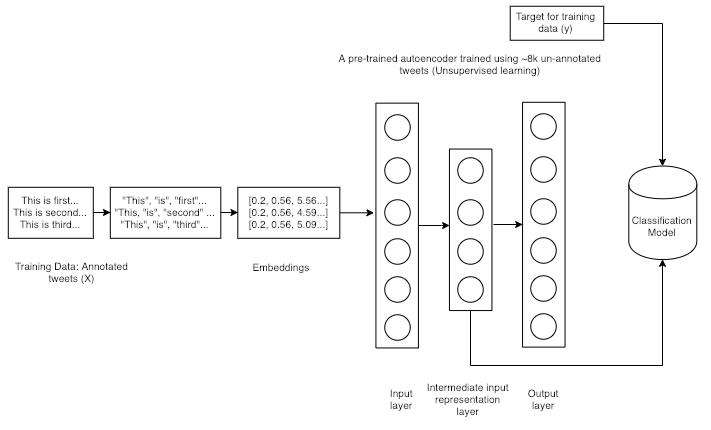
\includegraphics[width=\linewidth]{ae2.png}
    \caption{Autoencoder}
    \label{fig:my_label}
\end{figure}

An autoencoder is an unsupervised learning method which is used for compressing the high dimensional input data. It could also be used in tasks of dimensionality reduction for the same reason.
An autoencoder attempts to reconstruct the input that was fed to it and does so by creating an intermediate representation. This intermediate representation is highly useful as it contains the concentrated, important, useful and relevant input.
\medskip\\
The autoencoder then attempts to reconstruct the initial input given this intermediate representation. An Autoencoder can also be contextualized as a machine containing an Encoder and a Decoder. The Encoder encodes the input the input into a low dimensional space so as to extract only relevant information from the inputs.
\medskip\\
The decoder then decodes this internal representation to reconstruct the input again.
Our dataset is 10k tweets, since we are dealing with textual data we first encode our words and sentences into floating point vectors so that our machine learning model is able to work.
\medskip\\
We use Keras, a Deep Learning library for Python, that is simple, modular, and extensible. TensorFlow background for our Autoencoder implementation. We propose an Autoencoder model which learns input representation of our sentence tweets. We then train an Autoencoder using 8k unlabelled tweets. We then input the 2k annotated tweets to the trained Autoencoder and extract the floating point numpy array representation of my input data by getting the intermediate output of the Encoder layer.


We have defined our Autoencoder as having following layers:
\begin{itemize}
    \item Embeddings Layer: The embeddings layer in keras, is a default layer that converts words into floating point vectors suitable for machine learning computations.
    \item Flatten Layer: This layer flattens the array that it gets as input.
    \item Dense Layer: A dense layer with Relu activation and 32 neurons.
    \item Dense Layer: A dense layer with Sigmoid activation and 16 neurons.
    \item Dense Layer: A dense layer with Sigmoid activation and 16 neurons.
    \item Dense Layer: A dense layer with tan hyperbolic activation and 32 neurons.
    \item Dense Layer: A dense layer with Relu activation and 88 neurons.
\end{itemize}

We get a 2k X 32 array. For those 2k tweets we have a output label which we can feed into a classifier using Naive Bayes, Random Forests, Decision Trees, Support Vector Classifier and a Logistic Regression.
\newpage
\subsection{USING GOOGLE PRE - TRAINED WORD2VEC MODEL AND CLASSIFICATION MODELS }
\begin{figure}[ht]
    \centering
    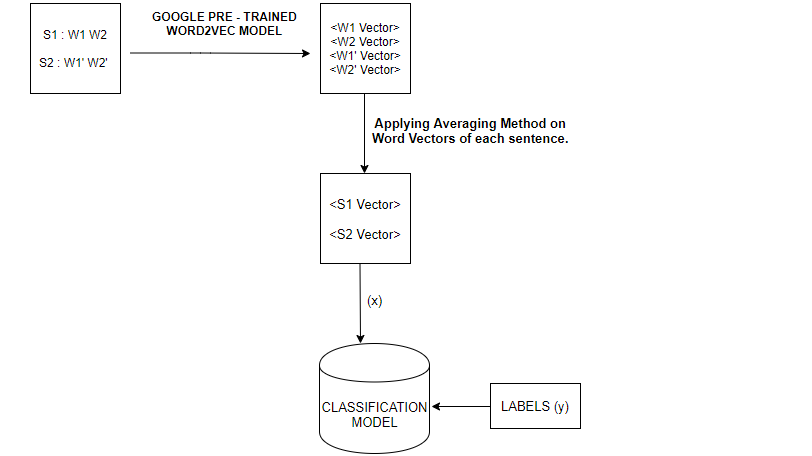
\includegraphics[width=\linewidth]{GooglePre-Trained.png}
    \caption{Google Pre-Trained Word2Vec Model}
    \label{fig:my_label}
\end{figure}

Google Pre-trained word2vec model provides us an implementation for computing the vector representations of the words. The model includes word vectors for a vocabulary of around 3 million words and phrases which are trained on about 100 billion words from a Google news dataset. The length of each vector is 300 features.These features are used in many natural language processing and machine learning applications.
\medskip\\
The model takes as input a word and produces the corresponding 300 length vector representation. Hence, for each word in a sentence a 300 length vector is produced. Taking it forward using the averaging method to produce a similar representation for the whole sentence, all these vectors obtained are combined and averaged so as to produce a 300 length vector which represents the whole sentence.
\medskip\\
The model is loaded using the gensim library. Gensim is an open source python library for doing natural language processing, with a main focus on topic modelling. It automatically extracts semantic topics from documents as efficiently as possible. The algorithms in the Gensim Library such as Word2Vec are unsupervised in nature.
\medskip\\
The sentence vectors are ultimately fed into classification models such as Naive Bayes, Random Forests, Decision Trees, Support Vector Classifier and Logistic Regression along with their labels using a 80/20 split for Training and Test data to determine the accuracy scores.


\newpage
\section{CONCLUSION}
\hrule
\vspace*{5mm}
The accuracy of the Long Short Term Memory unit is coming out to be 73.9\% for a data sample of ~1,200 rows.

\begin{figure}[ht]
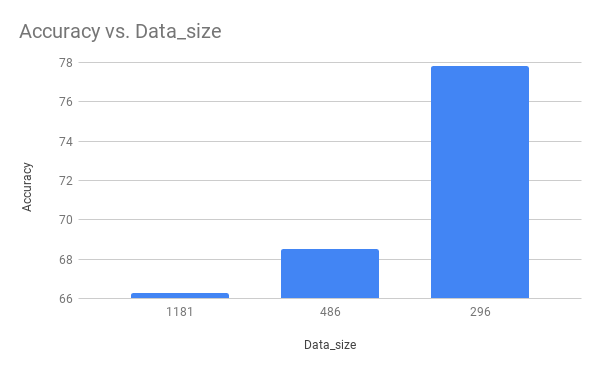
\includegraphics[width=\linewidth]{x1.png}
\caption{Accuracy vs Dataset size}
\end{figure}


\begin{figure}[!hb]
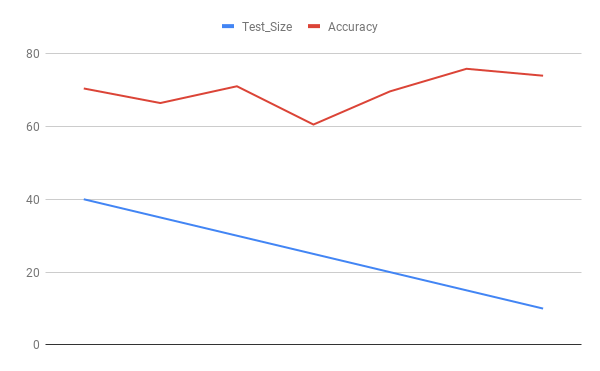
\includegraphics[width=\linewidth]{1.png}
\caption{Accuracy vs Testing sample size}
\end{figure}


\begin{figure}
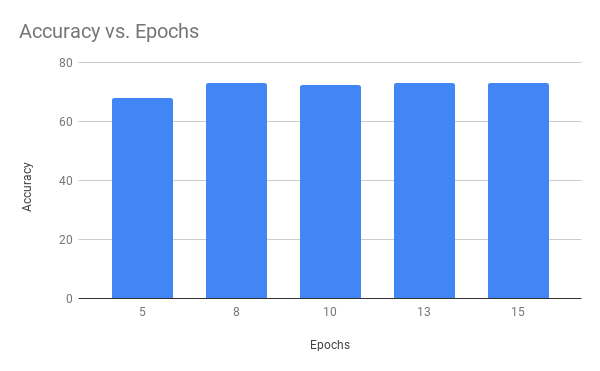
\includegraphics[width=\linewidth]{x3.png}
\caption{Accuracy vs Number of epochs}
\end{figure}


\begin{figure}
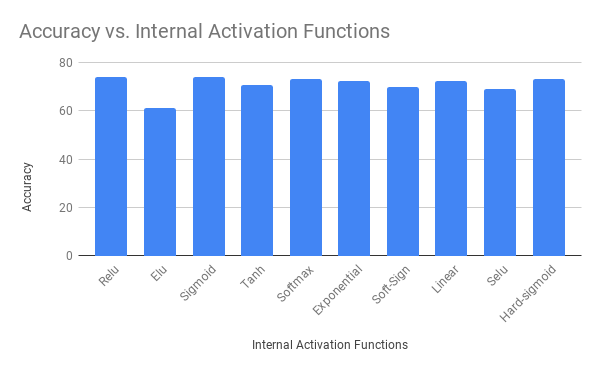
\includegraphics[width=\linewidth]{x4.png}
\caption{Accuracy vs Different Activation functions}
\end{figure}



\newpage 
\section{FUTURE WORK}
\hrule
\vspace*{5mm}
\begin{enumerate}
    \item \textit{Improving the accuracy of the present model :} The present model's accuracy can be improved by - 
    \begin{enumerate}
        \item Annotating more dataset and including the same for analysis done using Natural Language Processing.This would give more training data to the model and hence it would be able to predict with more accuracy.
        \item Using Word2Vec for vectorization of the words. Word2Vec is a more efficient approach and hence would increase the efficiency of the model.
        \item Tuning parameters to better suit our model would help increase the accuracy of prediction.
    \end{enumerate}
    \vspace*{5mm}
    \item \textit{Integrating Hindi Language tweets:} Presently, the model is designed to work on only English tweets. Because training the model on Hindi tweets is a complex task due to the intrinsic nature of some words in a tweet.\\
    For example : "aap se na ho payega"\\
    Here the word "aap" in the tweet could refer to the AAP political party or the hindi word aap.\\
    Hence, we would try to improve our model to work and predict on Hindi Language as well.
    
    
    \vspace*{5mm}
    \item \textit{Multi-class classification :} Currently the model is fitted on binary data(0,1) for identifying whether a tweet is political or not. We would want to extend it to predict for different classes of political parties like - Anti - AAP, Anti - BJP, Anti - Congress, Pro - BJP, Pro - Congress, Pro - AAP.
    
\end{enumerate}


\newpage
\section{REFERENCES}
\hrule
\vspace*{5mm}

\bibliographystyle{IEEEtran}
\bibliography{refer} 

\iffalse
\begin{itemize}
  \cite{}
\end{itemize}
\fi


\end{document}
